\chapter{Coffee Time Analysis}
% TODO Review ---------
In this chapter, the specification of the implemented application is outlined. The analysis of similar applications was made to obtain ideas.  After analysis, the low fidelity prototype was created to outline the first vision of the final application. Next, the high-fidelity prototype, along with Nielsen's heuristics analysis and user testing, were made. At the end of the chapter, considered tools and services are briefly described which are used to implement the application. 

\section{Considered Application}

Coffee Time is an application focused on searching nearby cafes. Users should be able to search and find nearby cafes around them to decide which establishment to visit. Each cafe is displayed with information such as distance, user's reviews, photos, opening hours and more. 

Added value to this standard information is a feature so-called ``the tags''. These tags are user-added additional info which describes more precisely what given cafe offer or for example if that cafe allows pets inside. 

The set of tags is defined, and users can add these tags to the cafe.  Each tag can be reviewed by other users. These reviews are done through ``like'' and ``dislike'' functionality. The purpose of tag's reviews is to prevent outdated information or misleading information.  

The example of such a review can be ``User visited cafe which has tag 'dog friendly', but unfortunately this information was incorrect. Consequently, the user decided to open the application and review the cafe's tag 'dog friendly' with dislike.''

Together with likes and dislikes, each tag has a computed score.  Each like gives to score plus one and as an opposite, dislike minus one. 
If any tags reach the score to -4, the tag is removed from the cafe, more precisely is not shown anymore to users. 
If such removed tag is proposed by any user again, it obtains "like" review. Thus score is incremented to -3 and is shown again. 

The application is location-based and offers a map view to support the convenience user experience. Google Places API as a data source is considered. Any cafe can be marked as user's favourite to give a faster way to find cafe whenever the user wants. 

To conclusion, Coffee Time is application focused on one domain -- searching nearby cafes where to go to study, talk with friends or for example have a great coffee. The application should be simple to use with a clean user interface. 

\section{Use Cases}
From the specification above, the use cases and use case scenarios were formed. The use cases diagram is listed in \cref{fig:use_case} and shows every use cases from the user perspective. Technically there is the role of application administrator which can check control back-end or available application's tags, but it skipped due to not importance of application perspective. 

\begin{figure}[htp]
    \centering
    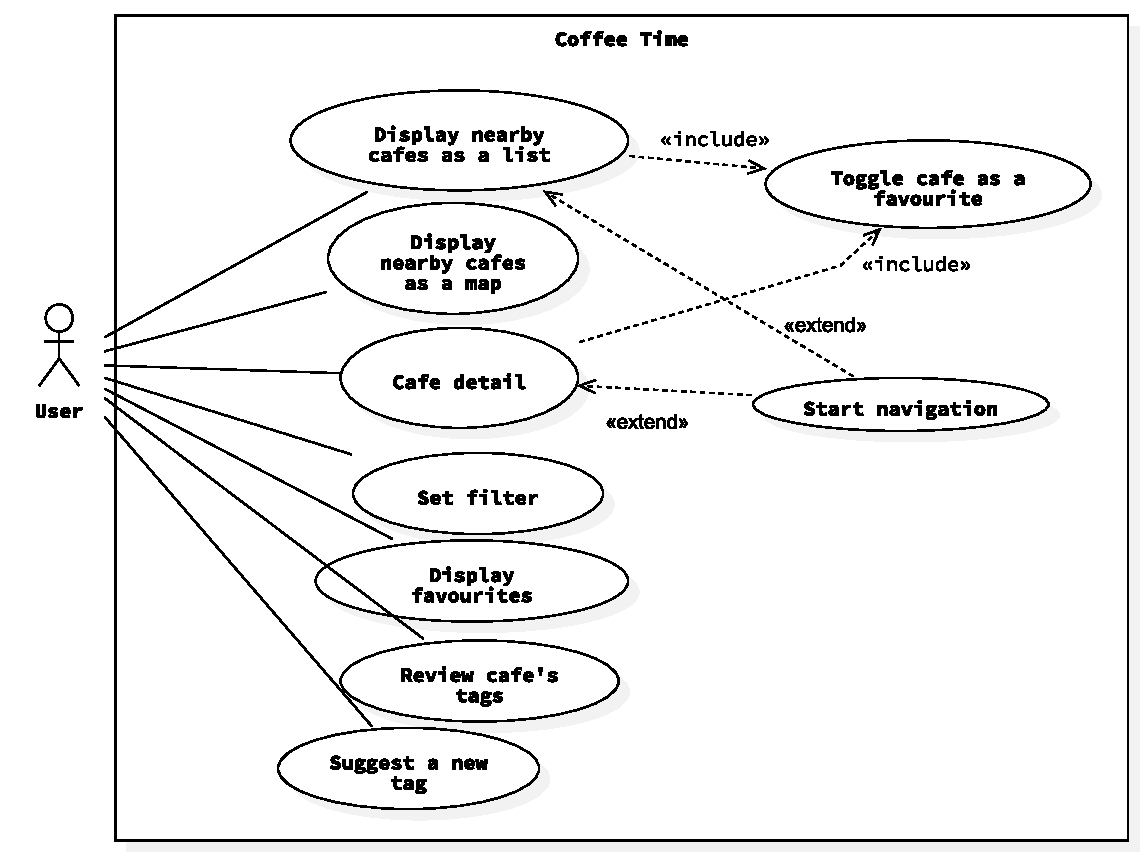
\includegraphics[width=\linewidth]{img/analysis/use_case.pdf}
    \caption{Application's use case diagram \todo{Add UC2 map}}
    \label{fig:use_case}
\end{figure}

As shown on diagram, the application has several use cases

\begin{itemize}
    \item UC1: Display nearby cafes as a list.
    \item UC2: Display nearby cafes as a list.
    \item UC3: Start navigation.
    \item UC4: Toggle cafe as a favourite.
    \item UC5: Setting the filter.
    \item UC6: Display favourite cafes.
    \item UC7: Review the cafe's tags.
    \item UC8: Suggest a new tag.
\end{itemize}

\subsection{UC1: Display Nearby Cafes As a List}
User can display nearby cafes in the form of the list view. The result is filtered by setting a filter, which can be altered by \textit{UC5}.

\textbf{Pre-Conditions} The user must be on the cafe list screen.

\newpara
\textbf{Basic Flow}

\begin{enumerate}
    \item User launch Coffee Time and lands on cafe list.
    \item Cafe list shows nearby cafes around him. Each cafe is displayed in the form of a card.
    \item User can pull the list down to refresh results. 
    \item User taps on cafe's card and is redirected to the detail view.
\end{enumerate}

\textbf{Alternative flow 1} The user launch navigation to the selected cafe.

% -------------

\subsection{UC2: Display Nearby Cafes as Map}
User can display nearby cafes in the form of the map view. Each cafe is shown as a map marker.

\textbf{Pre-Conditions} The user must be on the map screen.

\newpara
\textbf{Basic Flow}

\begin{enumerate}
    \item User launch application and change screen to map view. 
    \item Nearby cafes are shown as markers.
    \item The user taps on the marker and is redirected to the detail screen.
\end{enumerate}

\textbf{Alternative flow 1} The user taps anywhere on the map to display nearby cafes on the selected location.

% -------------

\subsection{UC3: Start navigation}
Use case allows starting navigation to selected cafe through native navigation applications.

\textbf{Pre-Conditions} The navigation services must be enabled.

\newpara
\textbf{Basic Flow}

\begin{enumerate}
    \item The user selects the cafe.
    \item The user selects navigate action. 
    \item The system request to open navigation application is opened. 
    \item User enables navigation and is redirected to navigation application. 
\end{enumerate}

\textbf{Alternative flow 1} The user dismisses navigation request and cancels navigation.

% -------------


\subsection{UC4: Toggle cafe as a favourite}
Each cafe can be marked as a favourite to faster future access. 

\textbf{Pre-Conditions} The cafe must be loaded, that is visible to the user. The user must be either on the cafe list screen, detail screen or favourite screen. 

\newpara
\textbf{Basic Flow}

\begin{enumerate}
    \item User has a cafe which wants to toggle as a favourite.
    \item User toggles cafe as a favourite.
\end{enumerate}

% -------------

\subsection{UC5: Setting the filter}
User changes the filter settings to filter out the cafe results.

\textbf{Pre-Conditions} There are results to filter.

\newpara
\textbf{Basic Flow}

\begin{enumerate}
    \item User opens filter settings screen.
    \item If it is suitable user changes results ordering from ``by distance'' (default) to ``by popularity''.
    \item If it is suitable user changes opening hours filter.
    \item Add tags to filter by, if any.  
    \item Returns back to the previous screen
    \item The results are filtered with the chosen filter.
\end{enumerate}

% -------------

\subsection{UC6: Display favourite cafes}
Display every favourite cafe in the form of the list view. 

\textbf{Pre-Conditions} The user must be on the map screen.

\newpara
\textbf{Basic Flow}

\begin{enumerate}
    \item User displays favourite cafe list.
    \item After the cafe is selected, the user is redirected to the cafe's detail screen.
\end{enumerate}

\textbf{Alternative flow 1} The user launches navigation to the selected cafe.

\textbf{Alternative flow 2} The user toggles cafe as not-favourite anymore.

% -------------

\subsection{UC7: Review the cafe's tags}
Use case allows users to review the cafe's tags with likes and dislikes. 

\textbf{Pre-Conditions} Cafe must have tags to review.  User must be on the cafe's detail screen.

\newpara
\textbf{Basic Flow}

\begin{enumerate}
    \item The user wants to suggest a change to the selected cafe.
    \item User reviews each tag with 'like', 'dislike' or skip review for the given tag. 
    \item User confirms review.
\end{enumerate}

\textbf{Alternative flow 1} The user decides not to do the review and goes back to the detail screen.

% -------------

\subsection{UC8:  Suggest a new tag}
Use case allows users to suggest a new tag to the selected cafe.

\textbf{Pre-Conditions} Cafe must have tags to review.  User must be on the cafe's detail screen.

\newpara
\textbf{Basic Flow}

\begin{enumerate}
    \item The user wants to suggest a change to the selected cafe.
    \item The user selects new tags for the suggestion. 
    \item The user confirms the suggestion.
\end{enumerate}

\textbf{Alternative flow 1} The user decides not to make the suggestion and goes back to the detail screen.

% -------------

\todo{conclusion for use cases?}

% TODO ---- End Review ---------

\section{Existing Alternatives}
The analysis of existing alternatives was made to research already created applications with similar features. Existing applications were searched through Android's official store. Applications with these functionalities were chosen for the review.

\begin{itemize}
    \item Nearby place search
    \item Application's theme should be cafes or similar
\end{itemize}

For comparison five, the most inspiring and distinguish applications were chosen. The following lines briefly describe one of each, their target audience, the advantages and drawbacks. 

\subsection{Gastromapa Lukáše Hejlíka}
\todo{LINK}
Published in the first quarter of 2019 as a new application for exploring restaurants in the Czech Republic.  The application's speciality is that restaurants' reviews are not done by users but by gastronomy specialist \textit{Lukáš~Hejlík}.

As soon as the application launches, it displays nearby restaurants. Each establishment is shown as a card with important information such as an address, distance and type of restaurant. The main card's domain is a large photo which should catch the user's eye to take a look. 

After the card is clicked, the user is presented with the restaurant's detail, where more information such as opening hours, map location and comprehensive review by~\textit{L.~Hejlík} can be found. From this detail navigation to the chosen restaurant can be launched. The target audience is anyone who seeks to visit unknown places and possess the opportunity to taste great food.


\begin{figure}[h]
    \centering
    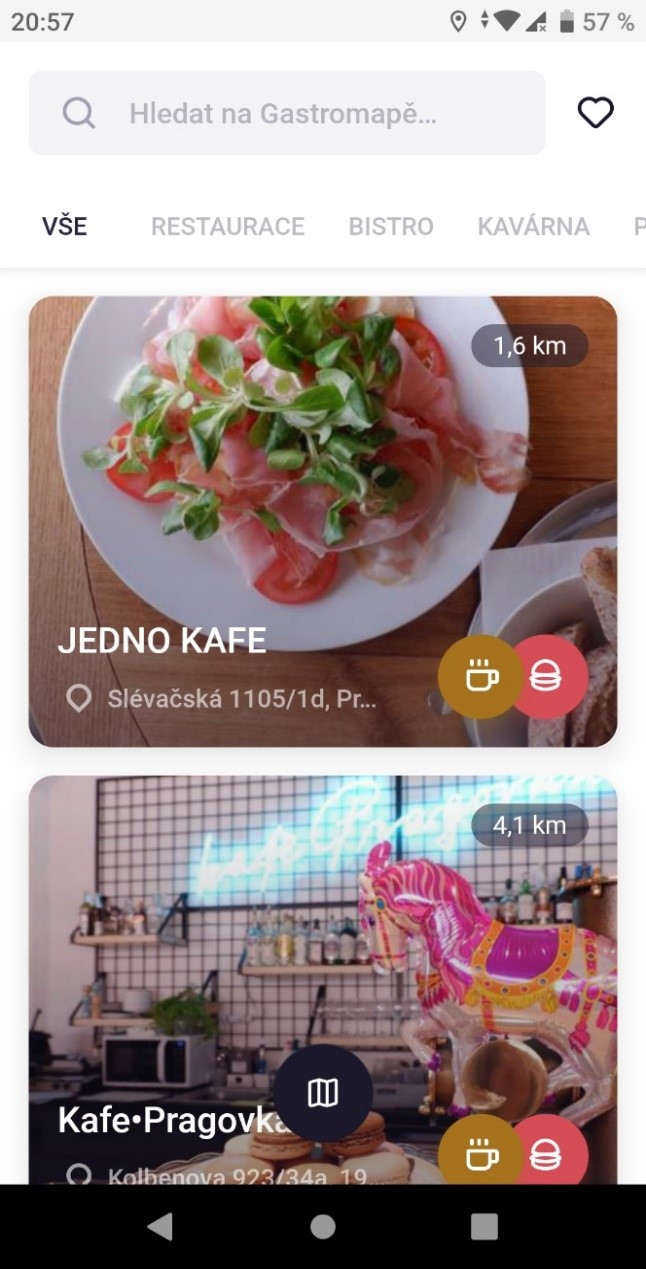
\includegraphics[width=0.33\linewidth]{img/analysis/gastromapa_hejlik.jpg}
    \caption{Gastromapa \textit{L. Hejlíka} \todo{Include app's images?}}
    \label{fig:gastromapa-hejlik}
\end{figure}

\subsubsection{The advantages}
\begin{itemize}
    \item Design is fresh, clean and users can immediately see relevant content.
    \item Thanks to clean design application is easy to use and understand.
    \item The whole application behaves smoothly without any noticeable freezing.
\end{itemize}

\subsubsection{The drawbacks}
\begin{itemize}
    \item The navigation button has a blackish colour that after scrolling disappears. If the restaurant has a darker photo, the button is hard to notice. 
    \item When coming back to the main screen, loading of the list is started again, and the previous search is lost.
    \item Detail screen on entry is fully covered with restaurant photo. From a design point of view, it is a nice touch, but users must scroll to see any information. 
\end{itemize}

\subsection{Pivní deník}
\todo{LINK} Application \textit{Pivní deník} is used to search nearby pubs in the Czech Republic and their beer offer. The content is created by the community, including served beer and their prices.  Application offers searching nearby restaurants filtered by beer brands. Each user can view a history of places they have visited, furthermore they can mark any pub as their favourite and share their experience.

\begin{figure}[h]
    \centering
    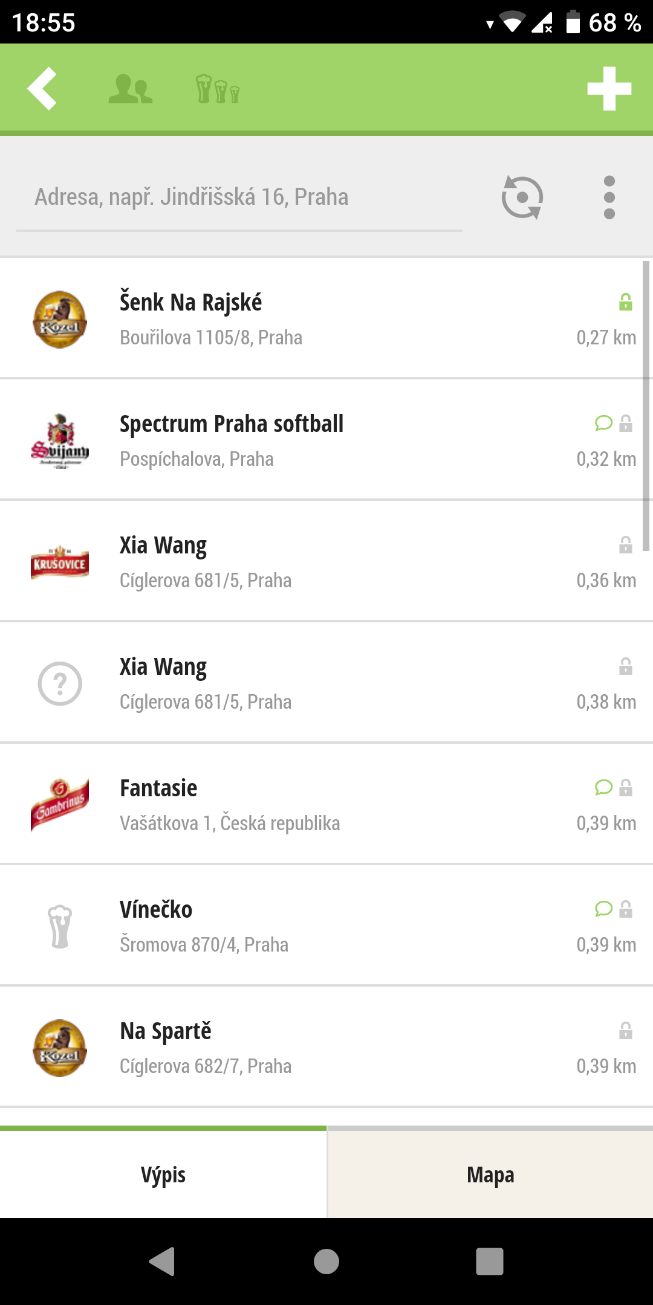
\includegraphics[width=0.33\linewidth]{img/analysis/pivni_denik.png}
    \caption{Pivní deník \todo{Include app's images?}}
    \label{fig:pivni-denik}
\end{figure}

\subsubsection{The advantages}
\begin{itemize}
    \item Pubs are displayed as a list or on the map.
    \item The served brands are displayed directly within the list, so it is not needed to visit details.
    \item The registration is optional for searching. If users want to contribute, they have to have an account.
\end{itemize}

\subsubsection{The drawbacks}
\begin{itemize}
    \item Registration can be done through Facebook or e-mail. With e-mail registration, the user is forced to leave the application and is redirected to the web page where registration is finished.
    \item As was said, content is created by the community. During the research, it was clear that many information is outdated or misleading. 
    \item Overall the application design looks outdated and does not meet current, modern,  trends.
    \item On the primary screen user's stats and at most three nearest pubs are displayed. The drawback is that on the larger screens, there is plenty of unused space. 
    \item Each restaurant displays only one brand of drafted beer. Nowadays, many pubs offer more than one brand. 
    \item Side menu can be opened only with the hamburger icon but not with slide to the right gesture.
\end{itemize}

\subsection{Restu}
\todo{LINK} Restu is another gastronomy guide focused on restaurants in the Czech Republic. Through this application reservations can be made. Application has many unique functionalities. For example ``discover'' section which shows attractive offers or the best cafe in the city. Another functionality is the ``check-in'' button which gives credits to the users if they eat at the given restaurant. Target audience is everyone who searches for new places where to eat and make a reservation.

\begin{figure}[h]
    \centering
    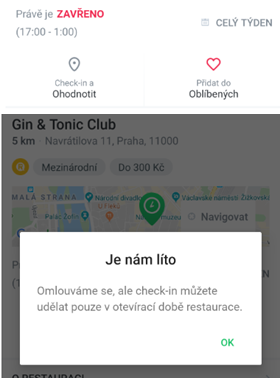
\includegraphics[width=0.33\linewidth]{img/analysis/restu.png}
    \caption{Restu \todo{change image}}
    \label{fig:restu}
\end{figure}

\subsubsection{The advantages}
\begin{itemize}
    \item Clean and well-structured layout.
    \item Opt-in registration.
\end{itemize}

\subsubsection{The drawbacks}
\begin{itemize}
    \item When a restaurant card is selected, window of the restaurant pops up but at the bottom cannot be hidden again.
    \item To review the restaurant, the user has to be signed in and the restaurant must be open. If the restaurant is closed, the review cannot be added.
\end{itemize}

\subsection{Zomato}
\todo{LINK} Zomato is primarily web-based restaurant browser in the world. It has its own database of establishments. Content is edited by users.  
On the primary screen are displayed ``week hits'', top restaurants or ``happy hours''. Restaurants are divided into categories such as ``Nightlife'' or ``Daily menu'' which helps for navigation within the application.
Target audience is anyone who wants to try new restaurants or someone who is looking for action offers. 

\begin{figure}[h]
    \centering
    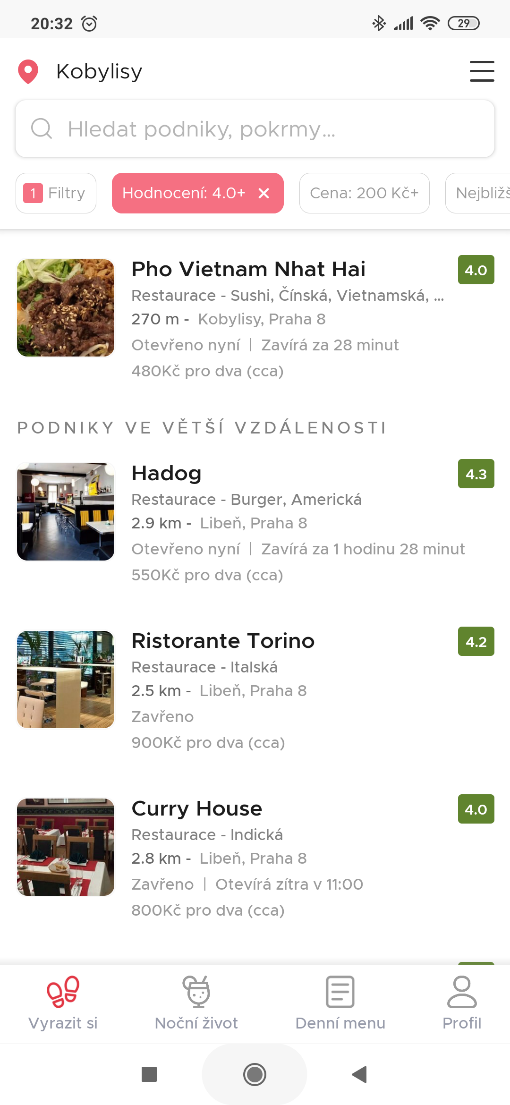
\includegraphics[width=0.33\linewidth]{img/analysis/zomato.png}
    \caption{Zomato}
    \label{fig:zomato}
\end{figure}

\subsubsection{The advantages}
\begin{itemize}
    \item Well solved filtering. Filter setting is intuitive, displays most used filters. 
    \item Advanced options for filtering with tags such as ``dog friendly'' or ``WiFi free''.
    \item Friendships with other users. If another user added review, notification is received.
\end{itemize}

\subsubsection{The drawbacks}
\begin{itemize}
    \item The primary screen is cluttered with many information at one place.
    \item Nearby restaurants list is hidden below ``favourites restaurants'' and ``month collections''.
    \item Full-text search in some circumstances behaves unexpectedly. For example, to search for restaurants which offer ``Asian food'' user has to type exactly ``asian'' but not ``asia''.
    \item Readability of some text is worsened by light background and greyish text colour. In some scenarios, it is hard to read.
\end{itemize}

\subsection{Google maps}
\todo{LINK} Popular worldwide map service by Google. One of the world's biggest database of places, restaurants. 
Google maps for each business, establishment displays additional info such as user reviews, photos, prices. 
Within Android system is already installed. Nearby places can be searched directly from the map. 

\begin{figure}[ht]
    \centering
    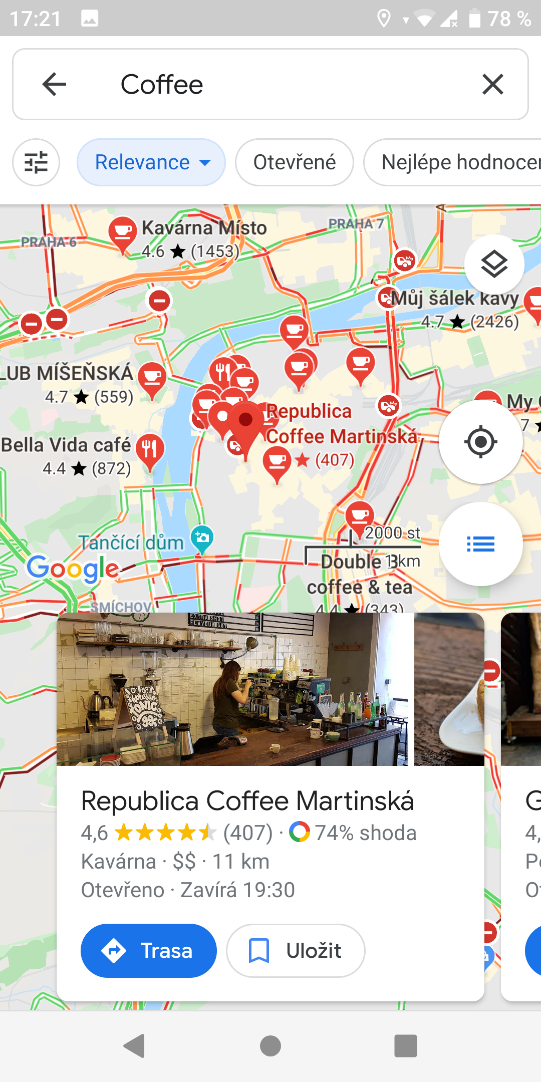
\includegraphics[width=0.33\linewidth]{img/analysis/gmaps.png}
    \caption{Google Maps}
    \label{fig:google-maps}
\end{figure}

\subsubsection{The advantages}
\begin{itemize}
    \item Well known and tested user interface which is embedded often to another application.
    \item No registration is required.
    \item Place detail includes plenty of useful information.
    \item GPS navigation with one click.
\end{itemize}

\subsubsection{The drawbacks}
\begin{itemize}
    \item Not domain focused, that means it does not offer focused content on particular businesses such as restaurants.
    \item No advanced filtering and result sorting.
\end{itemize}

To the conclusion, five applications were analysed on the Android system. Three apps are focused mainly on gastronomy. Another one specialises on beer. Last one, \textit{Google maps} is one of the most universal and robust. 
Each application has its own unique \gls{ui} \todo{not working gls, why??} and overall user experience differs. In the \cref{table:app-analysis} the targeted audience and user interface usefulness is summarised. \todo{review this}

\begin{table}[htbp]
\centering
\begin{tabular}{|l|l|l|}
\hline
\multicolumn{1}{|c|}{Application} & \multicolumn{1}{c|}{Targeted audience} & \multicolumn{1}{c|}{Overall \gls{ui}} \\ \hline
Gastromapa Lukáše hejlíka         & Everyone                               & Great                           \\ \hline
Pivní deník                       & Beer drinkers                          & Bad.                            \\ \hline
Restu                             & Everyone                               & Bad.                            \\ \hline
Zomato                            & Everyone                               & Good                            \\ \hline
Google                            & Everyone                               & Great but complex              \\ \hline
\end{tabular}
\caption{Analysed applications \gls{ui} summarization}
\label{table:app-analysis}
\end{table}


\section{Application prototype}

% TODO: REVIEW

One crucial step during the creation of software product is prototyping. Prototypes can help introduce different design ideas, can be easily tested, evaluated and changed. Prototyping techniques differ, but the desired output is the same -- provide visually concept of the final product. Prototypes do not help only visually, but they are part of user experience research and can find out which parts of the user interface should be changed before it is implemented.

There is no one correct definition of how prototypes should look and how they should be created. The prototype can be of the form as a simple sketch on paper to sophisticated pixel-perfect application~\cite{adobe-prototype}. Prototypes can be created multiple times during the whole creation process. 

In the early stages \gls{lofi} prototype is typically created. With \gls{lofi}, the application can be evaluated and user-tested if desired design concept is usable and understandable for users. When \gls{lofi} is finalised, the next prototype~--~\gls{hifi} is created. \gls{hifi} comes out from \gls{lofi} and should behave as fully functional application on the target platform. With \gls{hifi} once again, the application is evaluated with users and tested. 

To be more precise, according to \cite{adobe-prototype} \gls{lofi} prototype is a way to translate high-level concepts into tangible and testable artefacts. The most significant  functionality  of \gls{lofi} prototypes is to check and test the functionality of the product before visual appearance. Advantage of \gls{lofi} is that it is inexpensive, fast way to propose prototype. On the other hand, \gls{lofi} lacks complexity and cannot supply advanced interactivity. \gls{lofi} should be used to quickly create a prototype and get user feedback in the early stages of the creation process. 

After the~\gls{lofi} prototype, the \gls{hifi} is created. This prototype appears and function as similar as possible to the actual built application. \gls{hifi} should be created on the targeted platform and behave as it is the~final product. The goal is to have more complex \gls{ui} interactivity and have better feedback from user testing. Thanks to the fact that prototype looks like a real application user behaves more naturally and can get more precise a meaningful feedback than with \gls{lofi} prototype. 

To conclusion, \gls{lofi} prototypes are tested only internally with a small number of users and can be iterated more often and faster. While \gls{hifi} is more expensive to build and should be created and tested after \gls{lofi} prototype was accepted. On the other hand, \gls{hifi} gives better feedback from user testing, thus provides more valuable information.


\subsection{Coffee Time Prototype}
After the specification was written, next step was to create a \textit{task list}. The task list is written from the user's perspective that is, each task describe the user's action. It should tackle all important functionalities and even obvious one such as ``add record'' or ``remove record''.

\begin{figure}[htp]
    \centering
    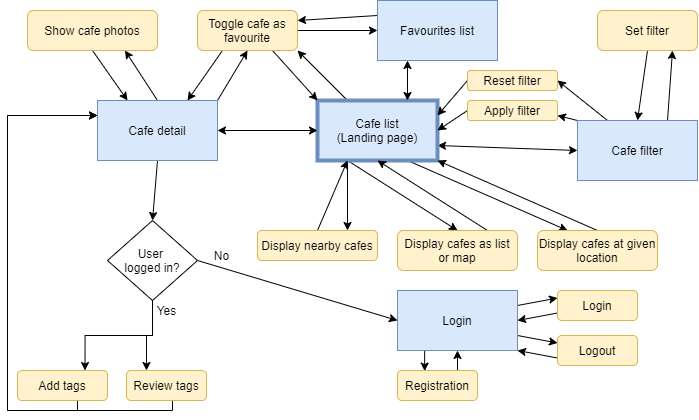
\includegraphics[width=0.9\textwidth]{img/analysis/task-list-graph.png}
    \caption{Coffee Time Task Graph}
    \label{fig:task-graph}
\end{figure}

Because the task list can become very long, it is usually transformed into a \textit{task graph}. The task graph does not have any specific definition, but it should contain every task along with each available screen within the application. Coffee Time's task graph is listed in \cref{fig:task-graph}. The blue rectangles are screens and the yellow ones are any task what users can do. The application's~entry point is highlighted with bold blue rectangle.

A note about \textit{User Interface Design (MI-NUR)} subject which was held during the winter semester of the academic year of 2019/2020. In this subject as a semester work was created the Coffee Time prototype. Sincere gratitude to classmates \textit{Bc. Ondřej John} and \textit{Bc. Vojtěch Polcar} for their co-working on the prototype. Furthermore, much appreciation to \textit{Ing. Jiří Hunka} for feedback and guidance during the work. The classmates helped during prototyping, proposing functionalities, researching and testing. The High-Fidelity prototype was implemented only by the thesis author. 

\subsubsection{Low Fidelity Prototype}
As a task graph was defined, the Lo-Fi prototype could be made. Although the application is considered as multi-platform application, the prototype was focused on Android, and its Material design \todo{Material LINK}. The inspiration was taken from typical Material layouts, such as AppBar with title and subsequent actions or tabs the bottom of the screen. 

First of all, the rough prototype was drawn on paper. Its purpose was to come up with some ideas and considered layout. After that, the Balsamiq \todo{link} prototyping software was used. The Balsamiq tries to mimic pencil and paper. The prototype is created with a set of components which looks like they were drawn by hand.
The most important feature was the ability to create deep links between screens or components. With a few clicks, the prototype was able to handle actions such as the open application menu or navigate to detail. With that tool, the clickable prototype focused on essential app's features was created. As a result, the PDF was exported. The PDF is enclosed as part of the thesis \todo{link to pdf}. The portion of the result is shown at \cref{fig:lofi}.

\begin{figure}[htp]
    \centering
    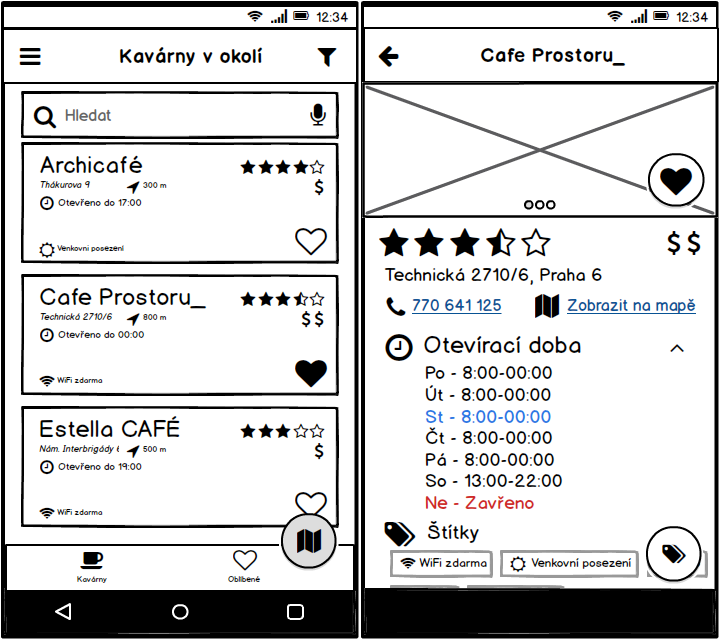
\includegraphics[width=0.9\textwidth]{img/analysis/lofi.png}
    \caption{\gls{lofi} prototype. Cafe list (left) and detail screen (right).}
    \label{fig:lofi}
\end{figure}

The result was tested with co-workers and closest author's family members. From the testing session, useful feedback was given, which is listed along with short answers. 

\begin{questions}
   \item On the cafe list, what if the cafe has more tags than it can display in the row. How to solve it? 
         \begin{answer}
          The solution is to calculate free screen space and display portion of available tags.
         \end{answer}

   \item Research more on how to solve user's reviews.
         \begin{answer}
         As a considered data source is Google Places API, it was acknowledged that it is not possible to add custom reviews through their API. \todo{link to answer that is not possible}.
         \end{answer}
    \item Navigation and contact buttons are too small. 
        \begin{answer}
        Taken into account during implementation.
        \end{answer}
    \item If the tag in detail is clicked, the cafe list with the given tag is shown.
        \begin{answer}
        Taken into account as a valuable tip.
        \end{answer}
    \item Focus on usability with mobile devices, mainly when the user's walk or are in public transport.
        \begin{answer}
        The usability should be more tested. 
        \end{answer}
    \item Focus more to provide understandable information about what tag is and how to use it.
     \begin{answer}
        Information and usability should be more revisited.
    \end{answer}
\end{questions}

\subsubsection{High Fidelity Prototype}
The \gls{hifi} prototype was created as Flutter application. Because of that, in the future, the already written code could be reused.  The goal was to create a fully functional prototype for Android devices. As was said earlier in this chapter, the goal of \gls{hifi} is provide an application which behaves as real one, which is mainly focused on user interface interaction. That means the application can be without any real communication whatsoever with back-end services. For Coffee Time there was prepared local JSON data source with randomly generated cafe names and their data. Besides that, a few, real one cafes were added to be less general and more known for potential testers.

\todo{LINK to prototype version} 
\todo{Prototype image}

\todo{User testing with others, video, results}

\todo{Any kind of information about prototype implementation?} 



\subsection{Nielsen Heuristic}
\todo{What is Nielsen Heuristic? Add link} 


\todo{Nielsen heuristic evaluation, results}

\todo{domain, architecture, tag state diagram, }

% TODO: \REVIEW ------------------------------------



\section{Technical analysis}

\subsection{Google Places API}
\todo{Google places API and how it is used.}

\section{Serverless approach \todo{Maybe move it to another chapter before analysis?}}

\todo{Firebase. Cloud functions. Firestore - NoSQL document based database. Pricing}
\blind[2]



